\documentclass{article}
\usepackage[utf8]{inputenc}
\usepackage{amssymb}
\usepackage{mathtools} 
\usepackage{geometry}
 \geometry{
 a4paper,
 total={140mm,227mm},
 left=35mm,
 top=35mm,
 }

\usepackage{float}
\usepackage{graphicx}
\usepackage{epstopdf}
\usepackage{amsmath}
\usepackage{bm}
\usepackage{color}

\setlength{\parindent}{0pt}
\numberwithin{figure}{section}
% equation number format: in section 1, (1.1), (1.2) ..
\usepackage{amsmath}
\numberwithin{equation}{section}

\makeatletter
% we use \prefix@<level> only if it is defined
\renewcommand{\@seccntformat}[1]{%
  \ifcsname prefix@#1\endcsname
    \csname prefix@#1\endcsname
  \else
    \csname the#1\endcsname\quad
  \fi}
% define \prefix@section
% \newcommand\prefix@section{}
\makeatother

%% multi col
\usepackage{multicol}

%% multi caption on subfigures
\usepackage{subcaption}

% hyperlinks
\usepackage{hyperref}
\hypersetup{
    colorlinks=true,
    linkcolor=black,   
    urlcolor=black,
    filecolor=black,
} 
\urlstyle{same}

% colored frames (boxes)
\usepackage{xcolor}
\usepackage{mdframed}

% vector arrow with \vv{ }
\usepackage{esvect}

%\hyphenpenalty 10000
%\exhyphenpenalty 10000
%\usepackage[none]{hyphenat}
%\usepackage[document]{ragged2e}

% strike through text
\usepackage[normalem]{ulem}
% \sout{Hello World}

%%%%%%%%%%%%%%%%%%
%% HEADER OVER %%%
%%%%%%%%%%%%%%%%%%

\usepackage{listings}
\lstset{language=Java,
basicstyle=\ttfamily,
keywordstyle=\color{blue}\ttfamily,
stringstyle=\color{red}\ttfamily,
commentstyle=\color{green}\ttfamily,
morecomment=[l][\color{magenta}]{\#}, 
%numbers=left,
numbersep=5pt, 
backgroundcolor=\color{white}, 
breaklines=true
}

\usepackage{siunitx}

\title{02101 Assignment 3}
\author{s144107 Roar Nind Steffensen\\s144063 Magnus Søborg-Madsen}
\date{\today}

\begin{document}
%\maketitle

\begin{titlepage}
\centering
\parindent=0pt
\newcommand{\HRule}{\rule{\textwidth}{1mm}}
 \HRule\\[1cm]\huge\textbf
{02101 Introductory Programming \\Assignment 3}\\[0.1cm]
\HRule\\[3cm]\vspace{-1 cm} \textbf{\Large{Group RR \& MGNS}}\\
\large{
Roar Nind Steffensen (s144107)\\
Magnus Middelboe Søborg-Madsen (s144063)}

\vspace{1 cm}

\begin{figure}[H]
\centering

\includegraphics[width=0.5\textwidth]{java.eps}
\label{fig:front}
\end{figure}

\vspace*{\stretch{2}} \normalsize %
Technical University of Denmark\\
\today
\vspace{0.5cm}
%\vspace*{-1cm}
\begin{figure}[h]
    \centering
    
\includegraphics[height=2cm]{DTUlogo.png}
\end{figure}
\end{titlepage}

\newpage
\setcounter{tocdepth}{2}

%\tableofcontents
%\vfill
\section*{Responsibility chart}

%We initially solved the problems individually to gain experience with problem solving in Java. Afterwards we compared our solutions, wrote the report together, and submitted our final (shared) Java code through CodeJudge. 

\begin{multicols}{2}

\begin{table}[H]
    \begin{tabular}{ll}
    \textbf{Java coding}      & \textbf{Main resp.} \\
    3.1 Functions & R       \\
    3.2 Traffic & both       \\
                &   \\
    \textbf{Comments}      & \textbf{Main resp.} \\
    3.1 Functions & both       \\
    3.2 Traffic & M        \\
    \end{tabular}
\end{table}

\begin{table}[H]
    \begin{tabular}{ll}
    \textbf{Report}      & \textbf{Main resp.} \\
    3.1 Functions & both       \\
    3.2 Traffic & both        \\
                &   \\
    \textbf{Figures}      & \textbf{Main resp.} \\
    3.1 Functions & both       \\
    3.2 Traffic & both        \\
    \end{tabular}
\end{table}

\end{multicols}

%\vspace{1 cm}

%% inputs

\section{Graphical function plotter}

The graphical function plotter is designed to take any of the implemented functions as input. This is obtained by creating an abstract \texttt{Function} super class, containing an \texttt{evaluate} method:

\begin{lstlisting}
public abstract double evaluate(double x);
\end{lstlisting}

By keeping the method abstract, each class extending the \texttt{Function} class must implement the method that evaluates the function for the argument \texttt{x}, and returns the value. 

The \texttt{Function} class is kept abstract since it would not make sense to evaluate or plot an unspecified function.\\
\\
We implemented the following subclasses by extending the superclass \texttt{Function}:

\subsection{\texttt{SineFunction}}
This function is implemented using the \texttt{sin(double a)} method from the \texttt{Math} class. The evaluate method (inherited from \texttt{Function}) returns the following:

\begin{lstlisting}
return a * Math.sin(b*x);
\end{lstlisting}

corresponding to the sine function $a \cdot \sin(b \cdot x)$, i.e. a sine wave with amplitude $a$, angular frequency $b$, and no phase shift. The requested example is shown in figure \ref{fig:f1}.

\begin{figure}[H]
    \begin{subfigure}{0.5\textwidth}
        \centering
    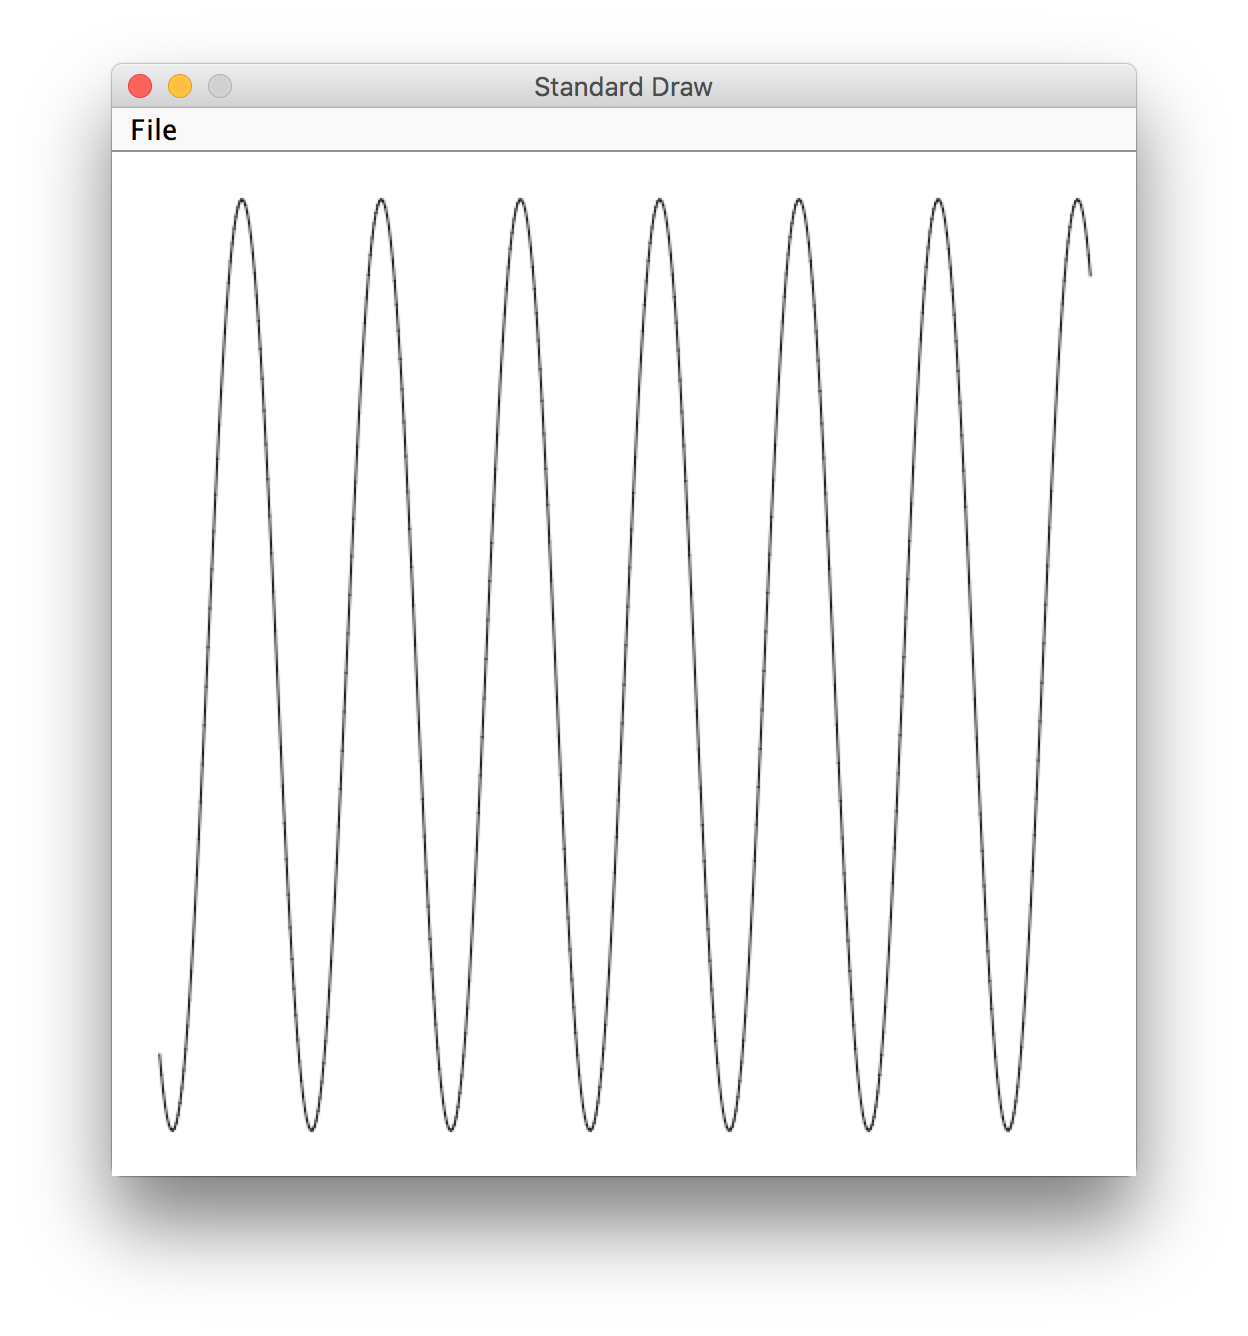
\includegraphics[width=0.7\linewidth]{GraphicalFunctionPlotter/fig/f1.png} 
    \caption{$f(x)=0.8\cdot \sin(2.1\cdot x)$.}
    \label{fig:f1}
    \end{subfigure}
    \begin{subfigure}{0.5\textwidth}
        \centering
    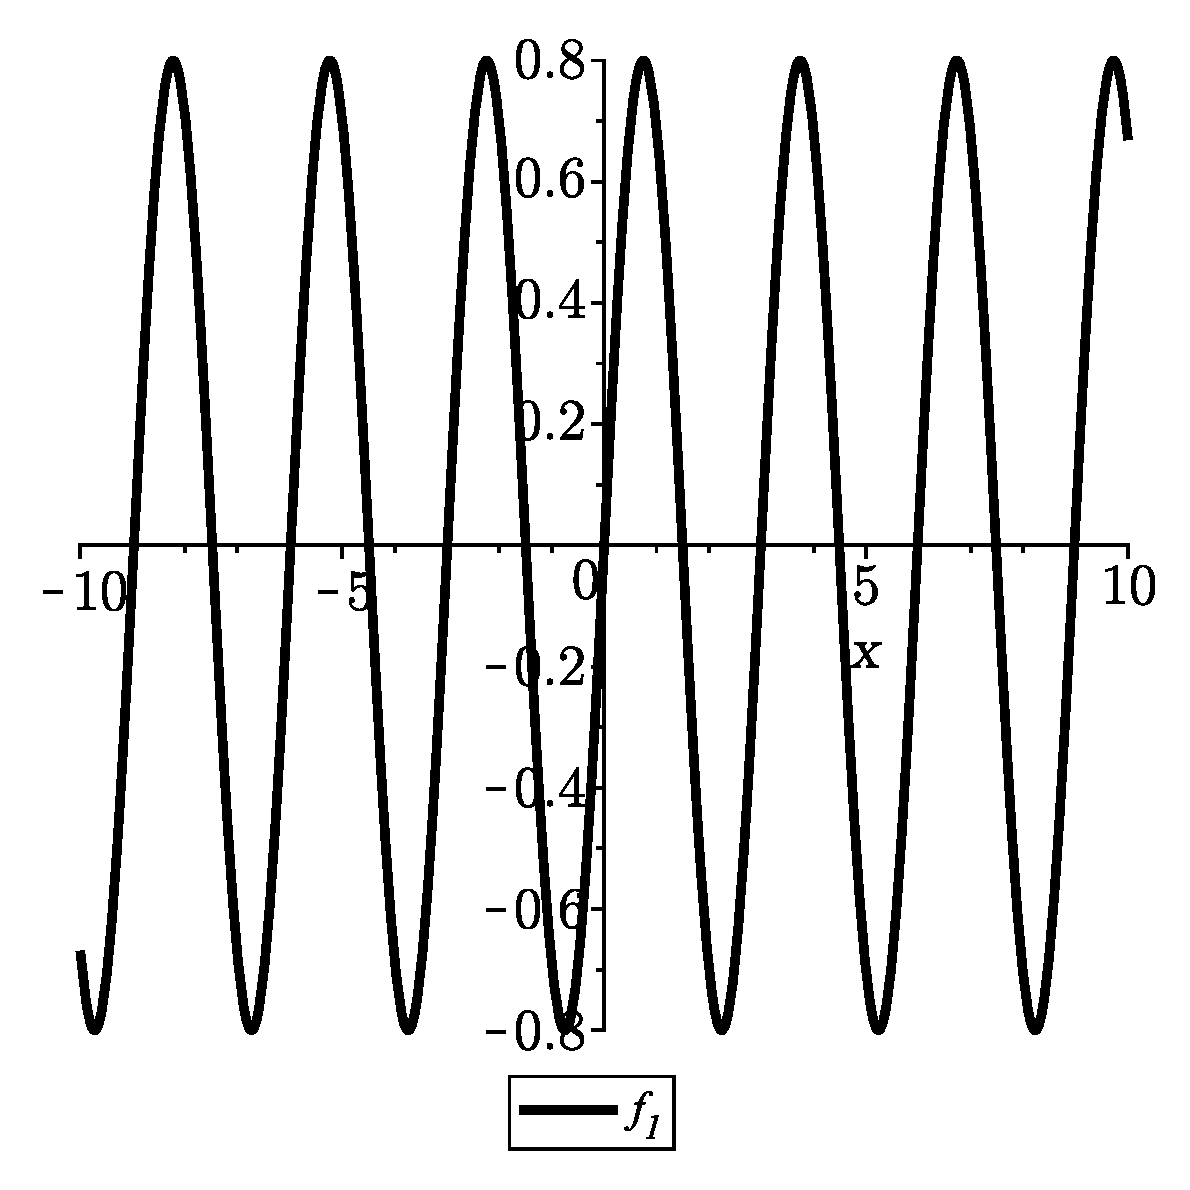
\includegraphics[width=0.7\linewidth]{GraphicalFunctionPlotter/fig/f1Check.eps}
    \caption{Same function plotted in Maple.}
    \label{fig:f1Check}
    \end{subfigure}
    \caption{Examples of the sine functions.}
\end{figure}
\newpage
\subsection{\texttt{PowerFunction}}
This function is implemented using the \texttt{pow(double a, double b)} method from the \texttt{Math} class. The \texttt{evaluate} method returns the following: 

\begin{lstlisting}
return b*Math.pow(Math.abs(x),a);
\end{lstlisting}

corresponding to the power function $b \cdot |x|^{a}$. The requested example is shown in figure \ref{fig:f2}. 


\begin{figure}[H]
    \begin{subfigure}{0.5\textwidth}
    \centering
    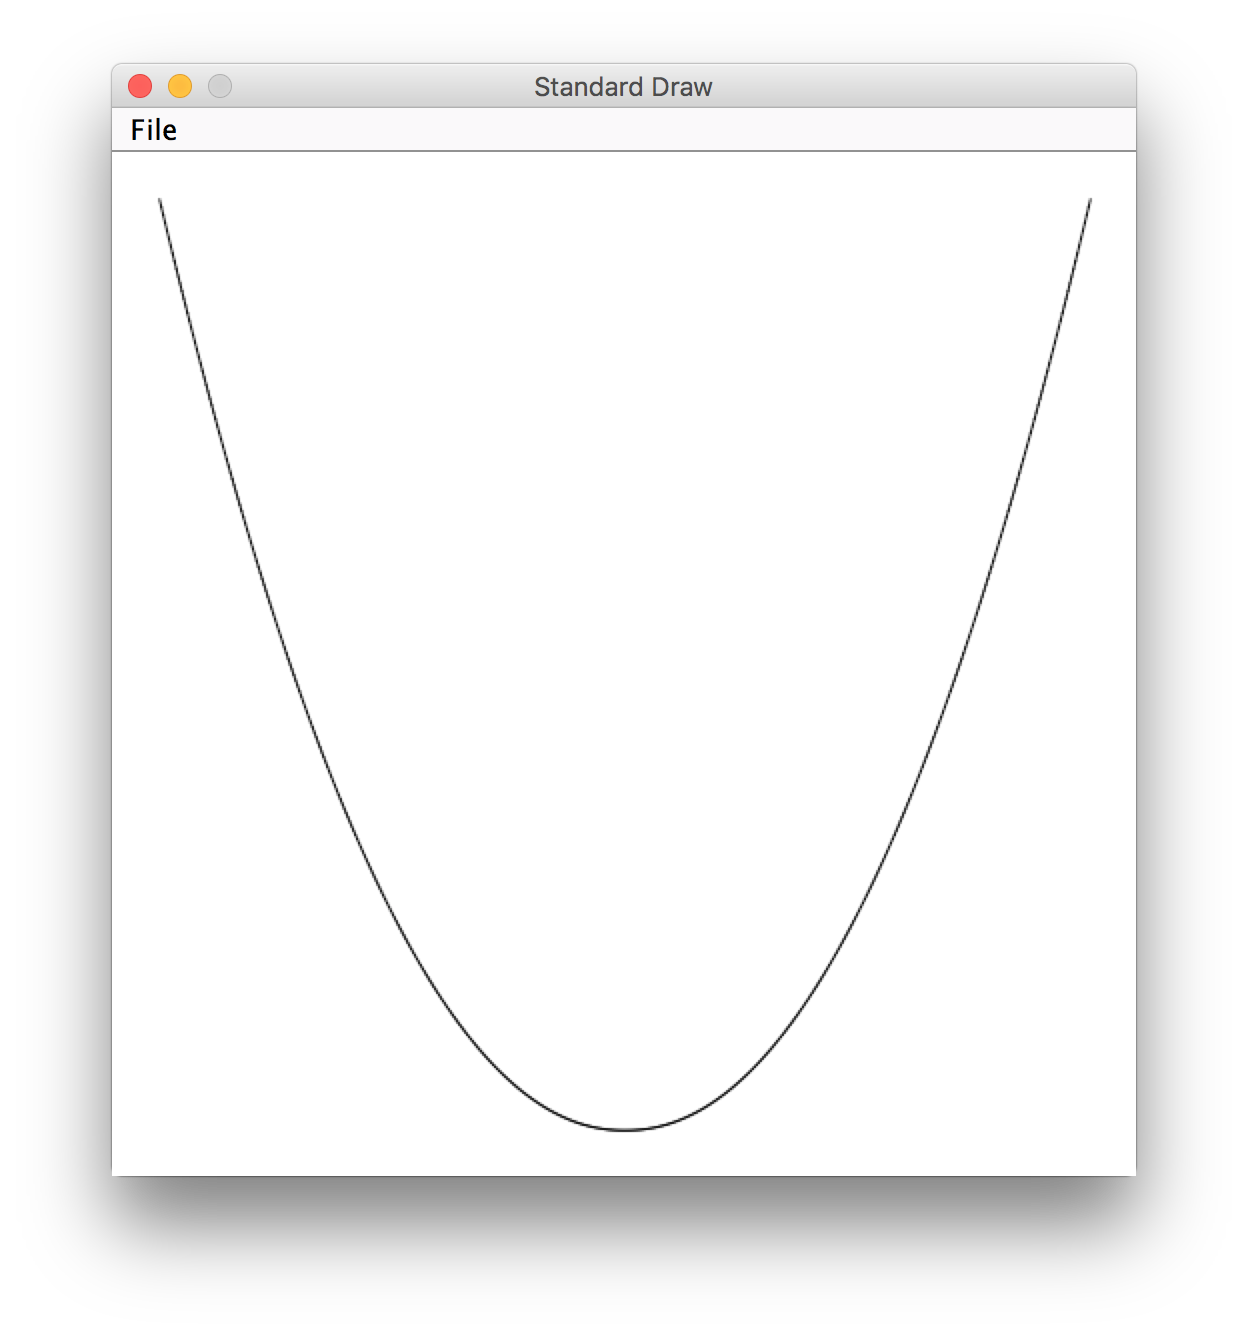
\includegraphics[width=0.7\linewidth]{GraphicalFunctionPlotter/fig/f2.png} 
    \caption{$f(x) = 2.1\cdot |x|^{2.0}$.}
    \label{fig:f2}
    \end{subfigure}
    \begin{subfigure}{0.5\textwidth}
    \centering
    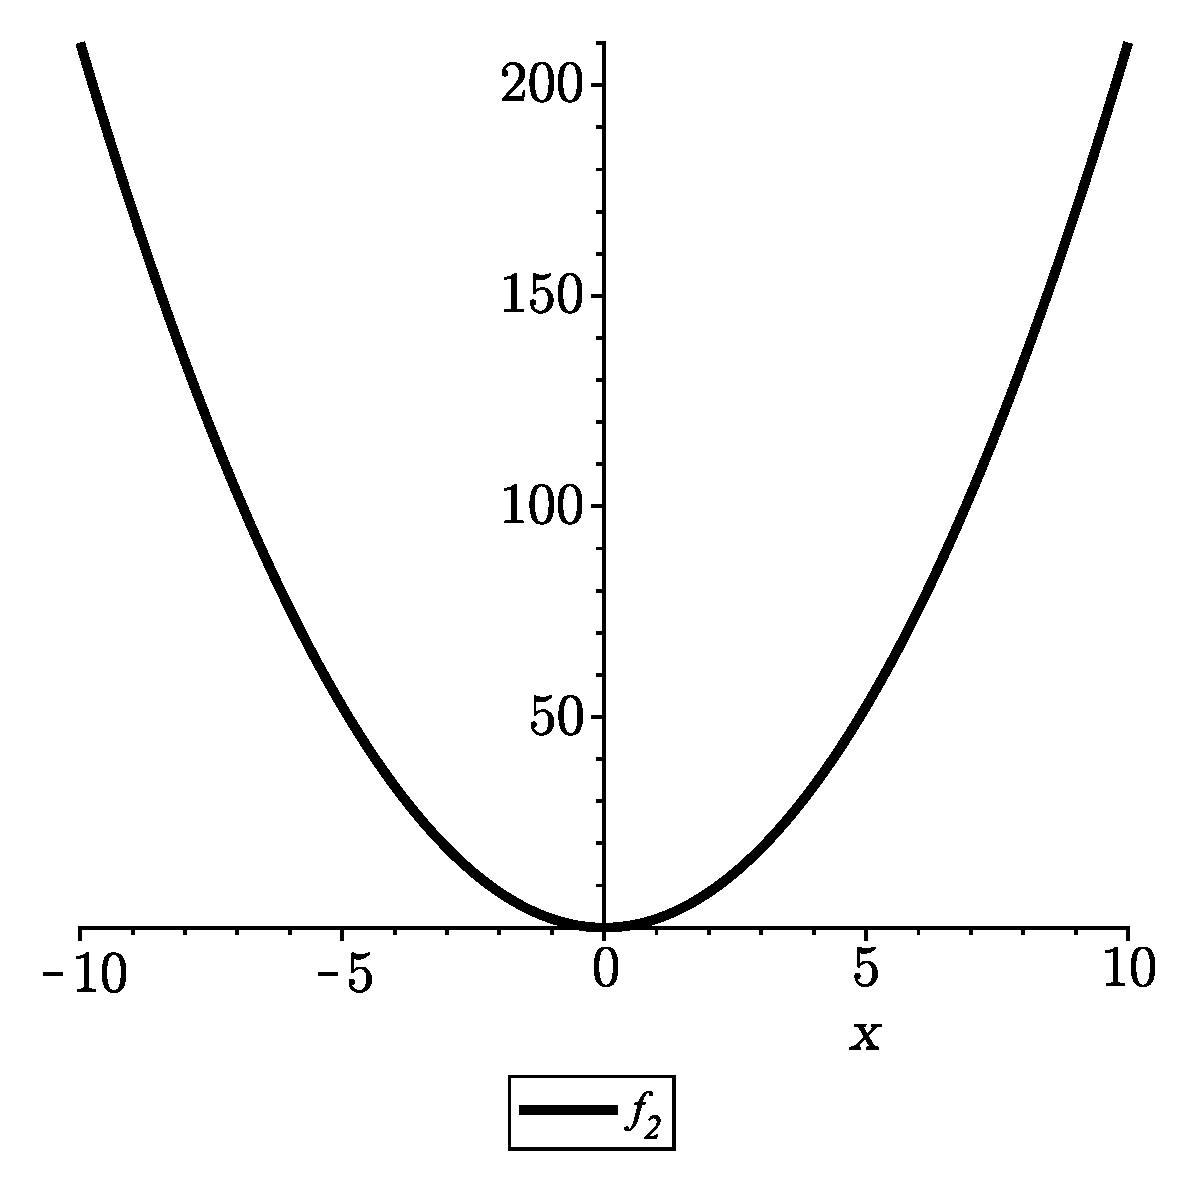
\includegraphics[width=0.7\linewidth]{GraphicalFunctionPlotter/fig/f2Check.eps}
    \caption{Same function plotted in Maple.}
    \label{fig:f2Check}
    \end{subfigure}
    \caption{Examples of the power functions.}
\end{figure}

\subsection{\texttt{ExponentialFunction}}
This function is also implemented using the \texttt{pow(double a, double b)} method from the \texttt{Math} class, as well as the built-in value of the constant e. The \texttt{evaluate} method returns the following:

\begin{lstlisting}
return a*Math.pow(Math.E,b*x);
\end{lstlisting}

corresponding to the exponential function $a \cdot \text{e}^{b \cdot x}$. \\
The requested example is shown in figure \ref{fig:f3}.

\begin{figure}[H]
    \begin{subfigure}{0.5\textwidth}
        \centering
        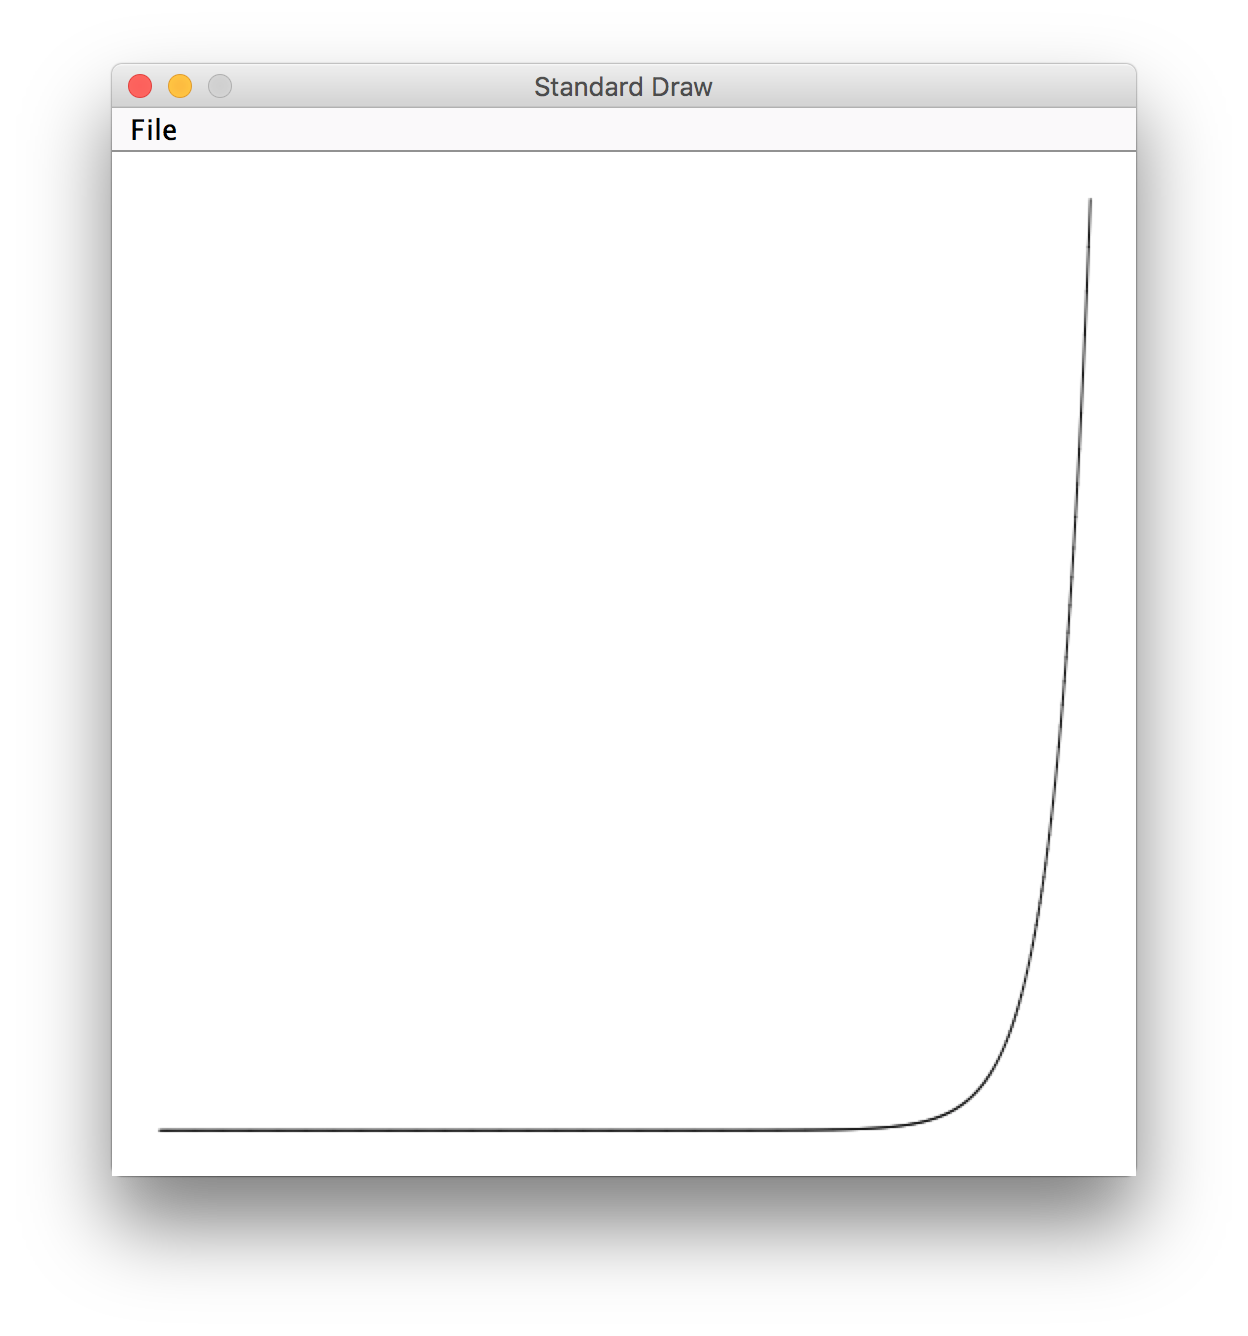
\includegraphics[width=0.7\linewidth]{GraphicalFunctionPlotter/fig/f3.png} 
        \caption{$f(x) = 3.2 \cdot \text{e}^{1.3 \cdot x}$.}
        \label{fig:f3}
    \end{subfigure}
    \begin{subfigure}{0.5\textwidth}
        \centering
        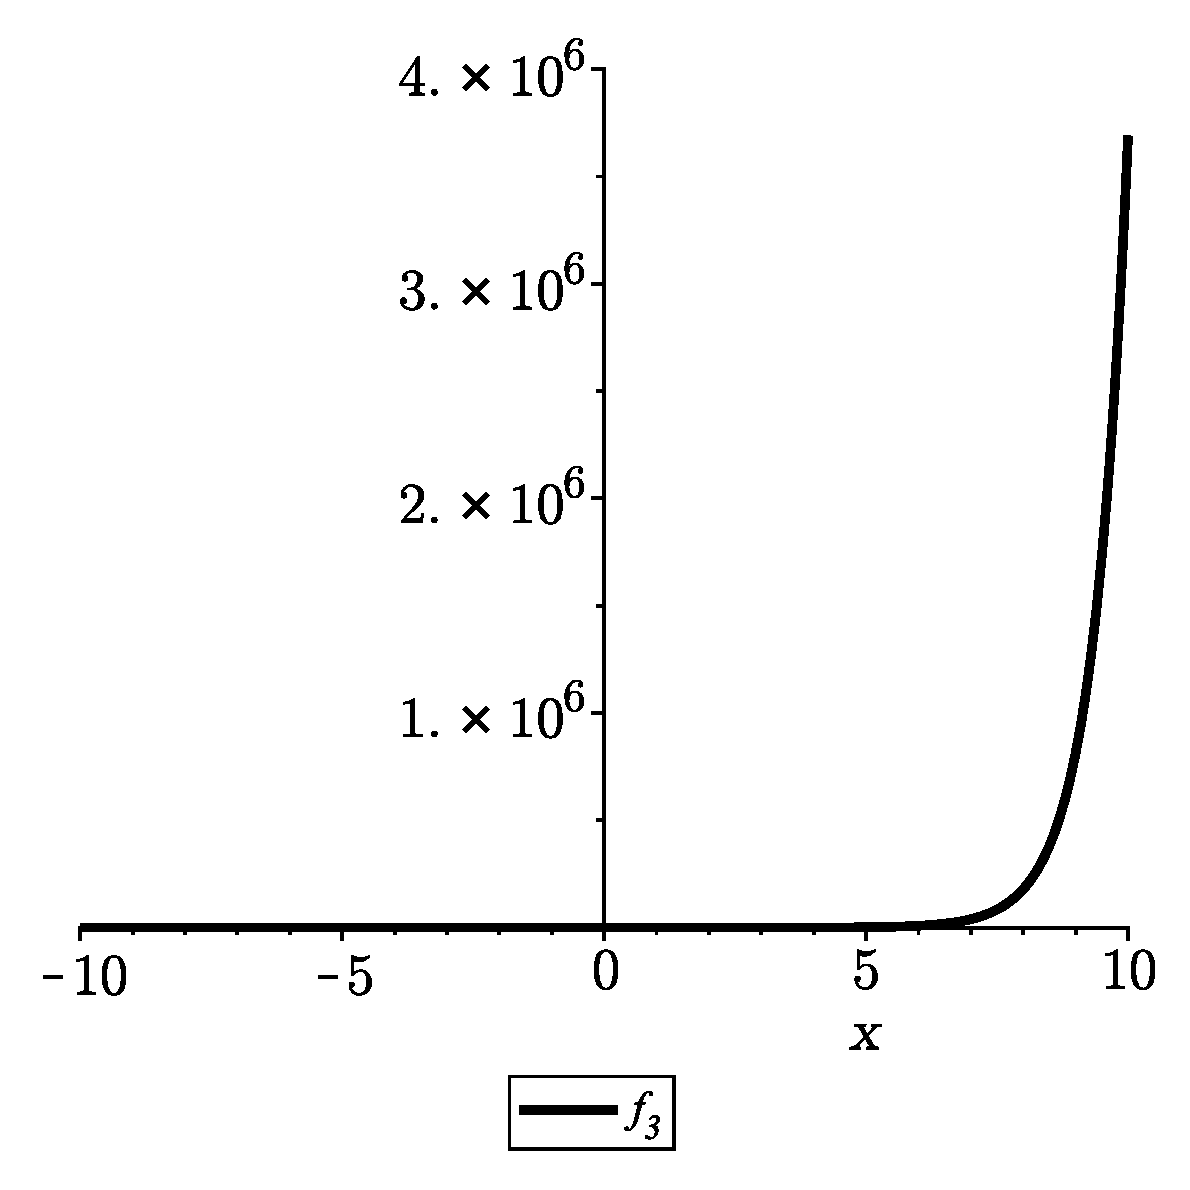
\includegraphics[width=0.7\linewidth]{GraphicalFunctionPlotter/fig/f3Check.eps}
        \caption{Same function plotted in Maple.}
        \label{fig:f3Check}
    \end{subfigure}
    \caption{Examples of the exponential functions.}
\end{figure}


\subsection{\texttt{PolynomialFunction}}
This function is also implemented using the \texttt{pow(double a, double b)} method from the \texttt{Math} class. The \texttt{evaluate} method returns the following:

\begin{lstlisting}
double sum = 0;
for(int i = 0; i < a.length; i++){
	sum += a[i]*Math.pow(x, i);
}
return sum;
\end{lstlisting}

Evaluating each value $a_n \cdot x^n$, returning the sum. \\
The requested examples are shown in figures \ref{fig:f4} and \ref{fig:f5}.

\begin{figure}[H]
    \begin{subfigure}{0.5\textwidth}
        \centering 
        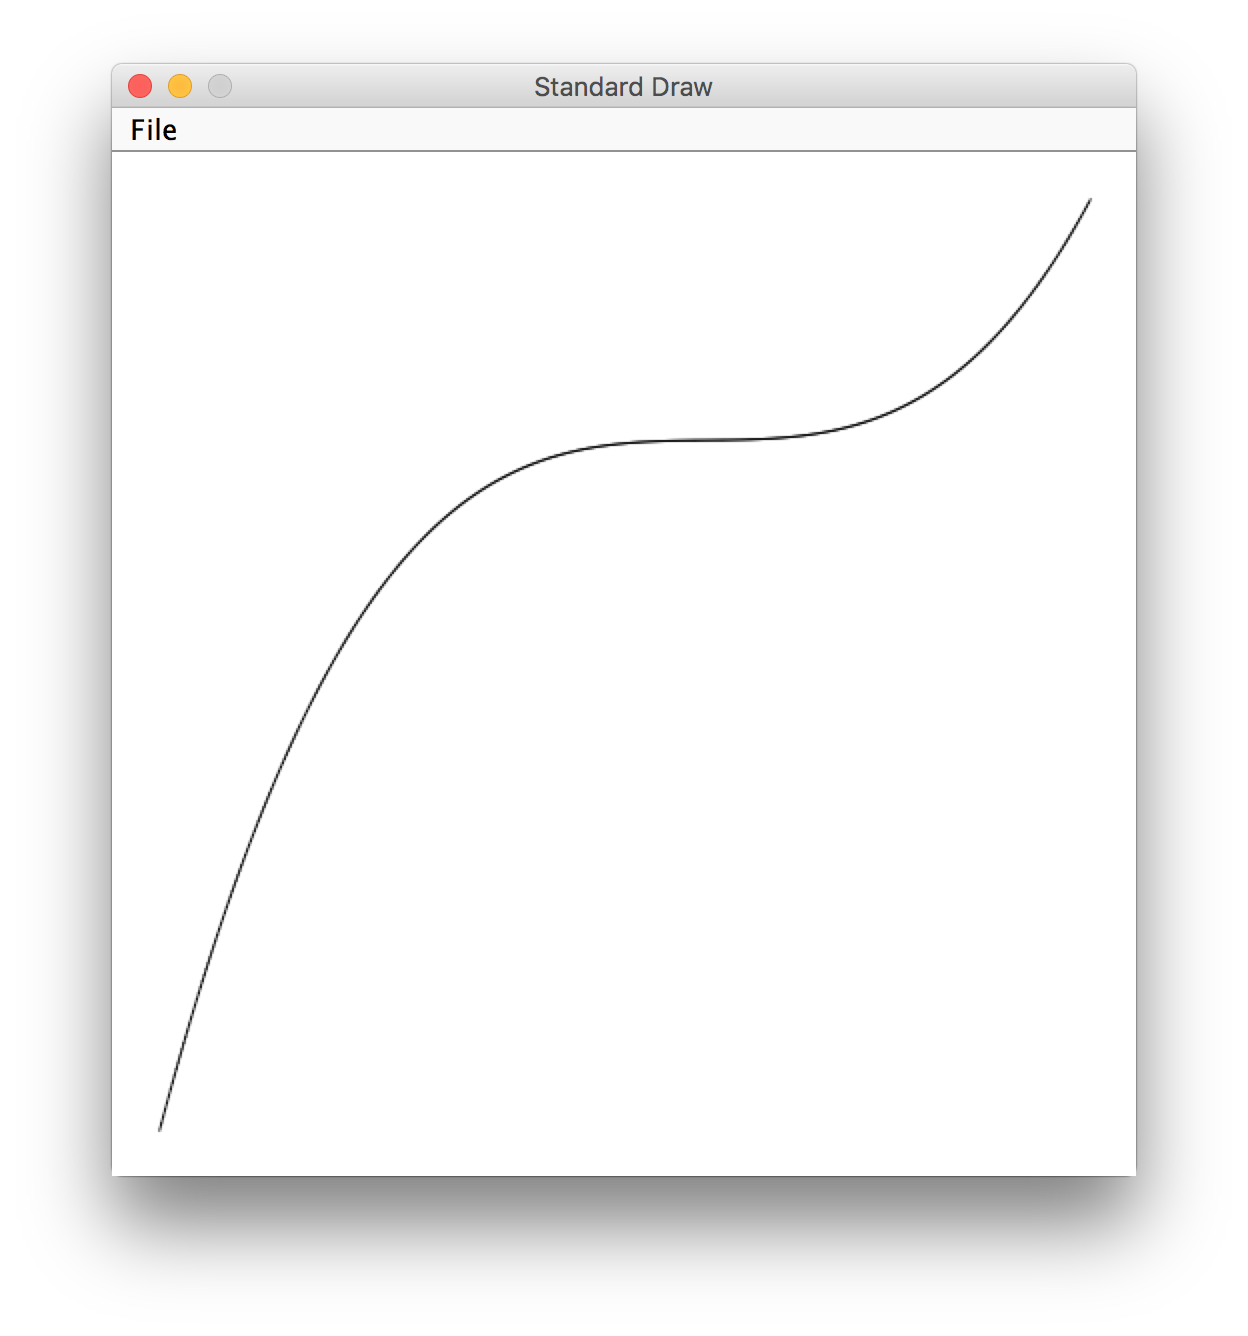
\includegraphics[width=0.7\linewidth]{GraphicalFunctionPlotter/fig/f4} 
        \caption{$f(x)=0.4x^3-2.1x^2+4.1x-3.1$.}
        \label{fig:f4}
    \end{subfigure}
    \begin{subfigure}{0.5\textwidth}
        \centering
        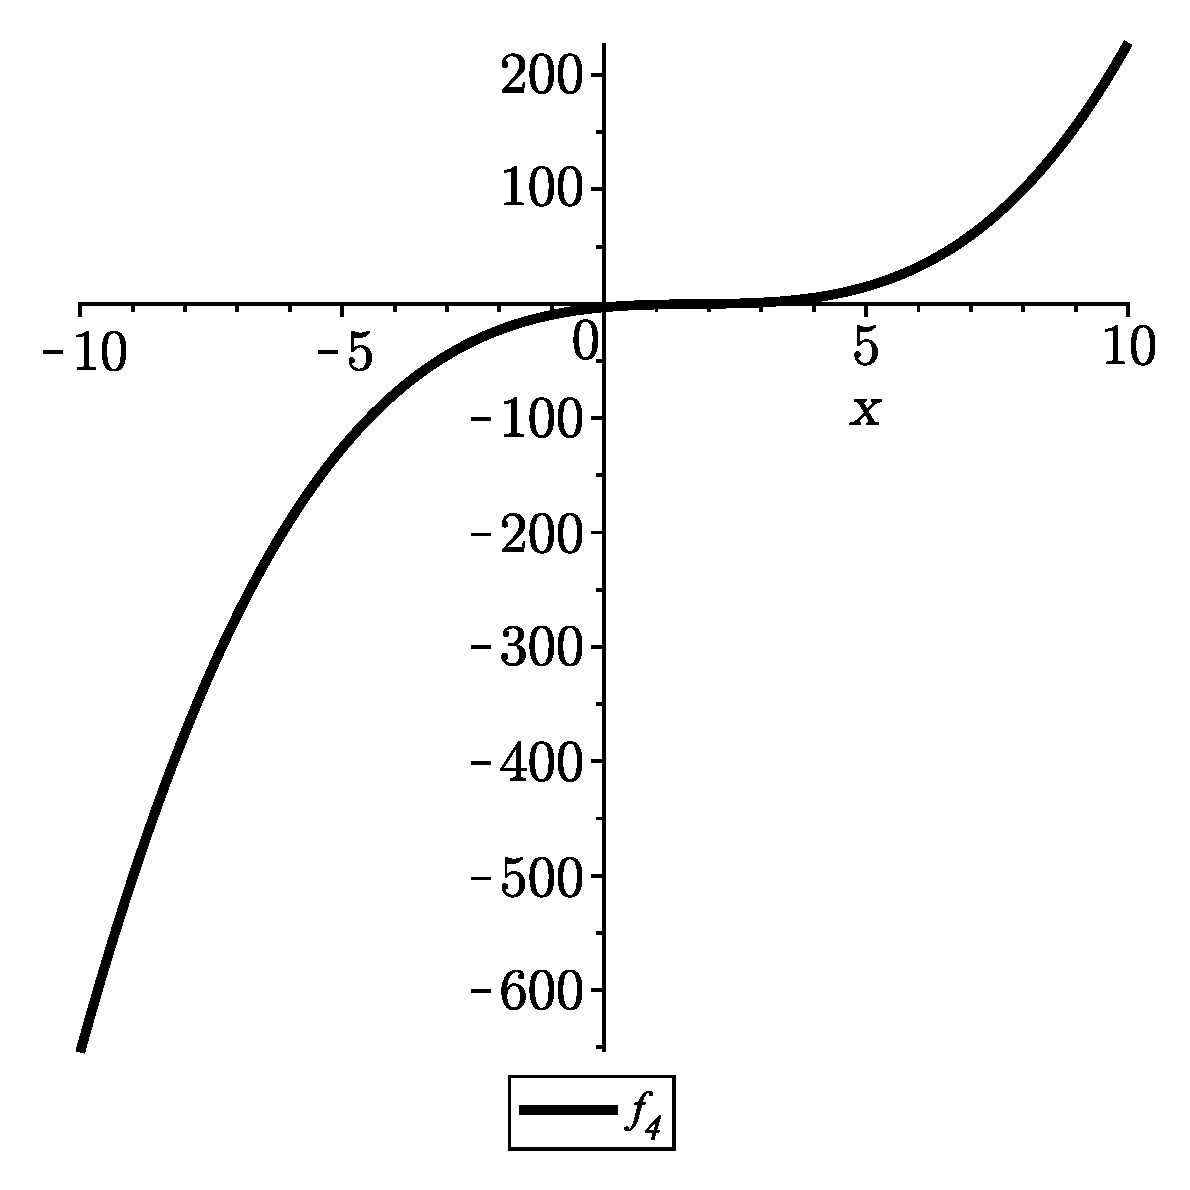
\includegraphics[width=0.7\linewidth]{GraphicalFunctionPlotter/fig/f4Check}
        \caption{Same function as \ref{fig:f4} plotted in Maple.}
        \label{fig:f4Check}
    \end{subfigure}
    \begin{subfigure}{0.5\textwidth}
        \centering
        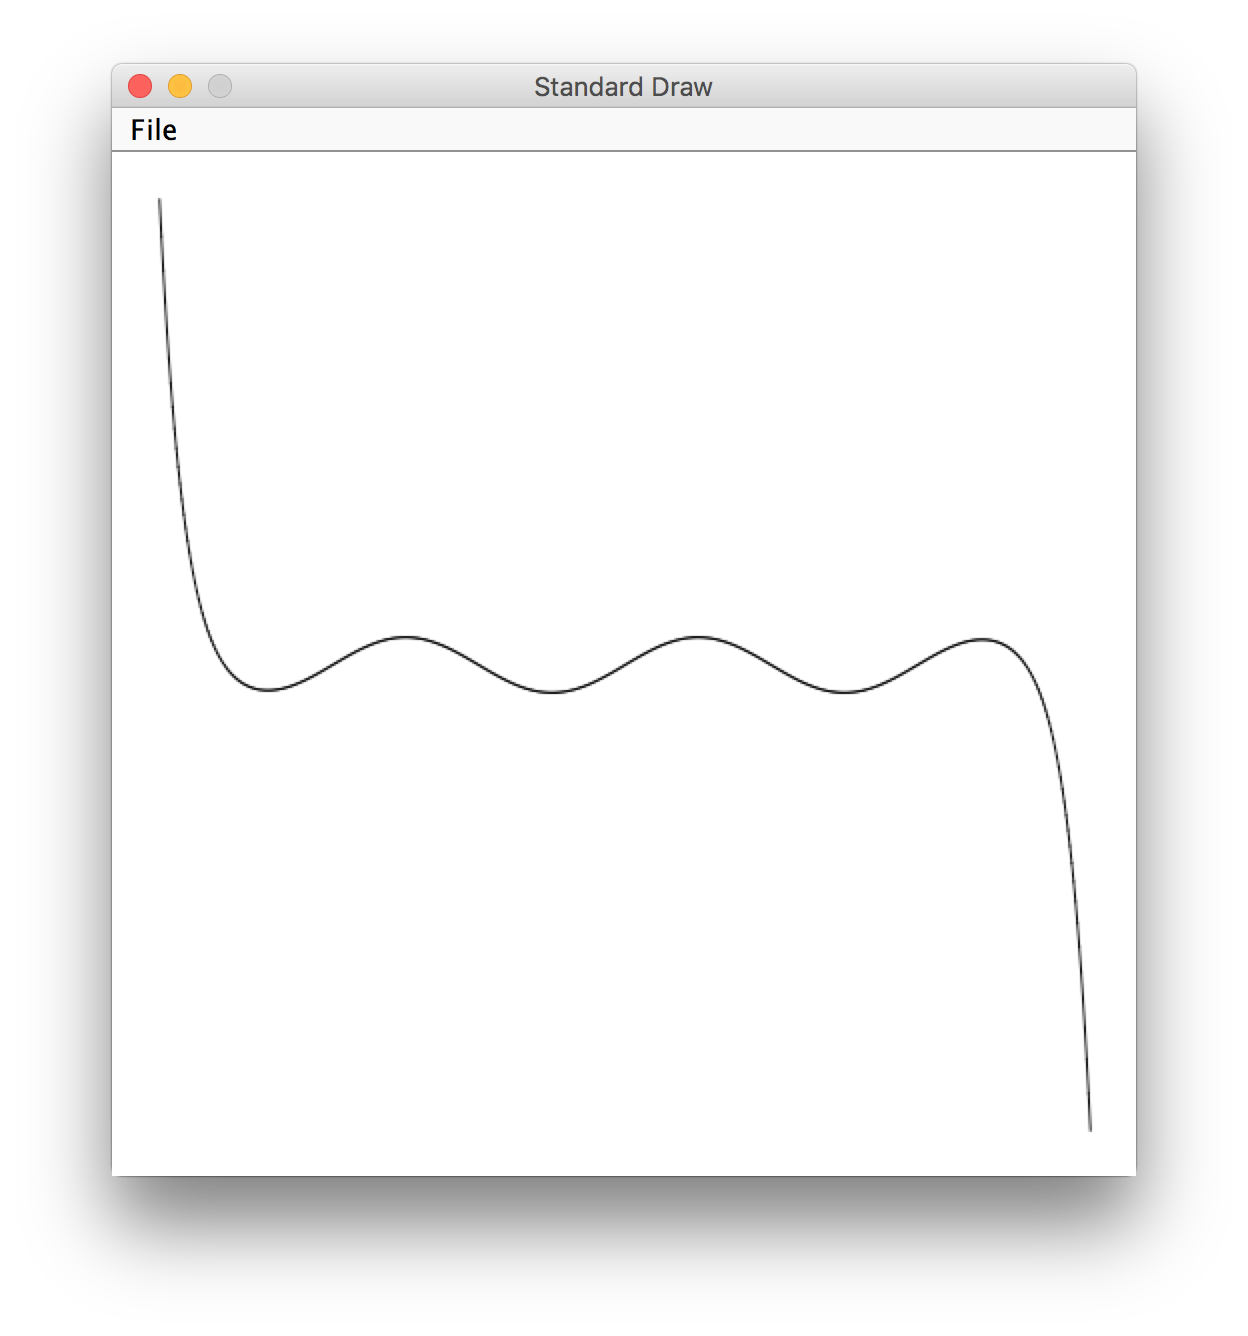
\includegraphics[width=0.7\linewidth]{GraphicalFunctionPlotter/fig/f5}
        \caption{Taylor expansion of a sine function, 19 degrees.}
        \label{fig:f5}
    \end{subfigure}
    \begin{subfigure}{0.5\textwidth}
        \centering
        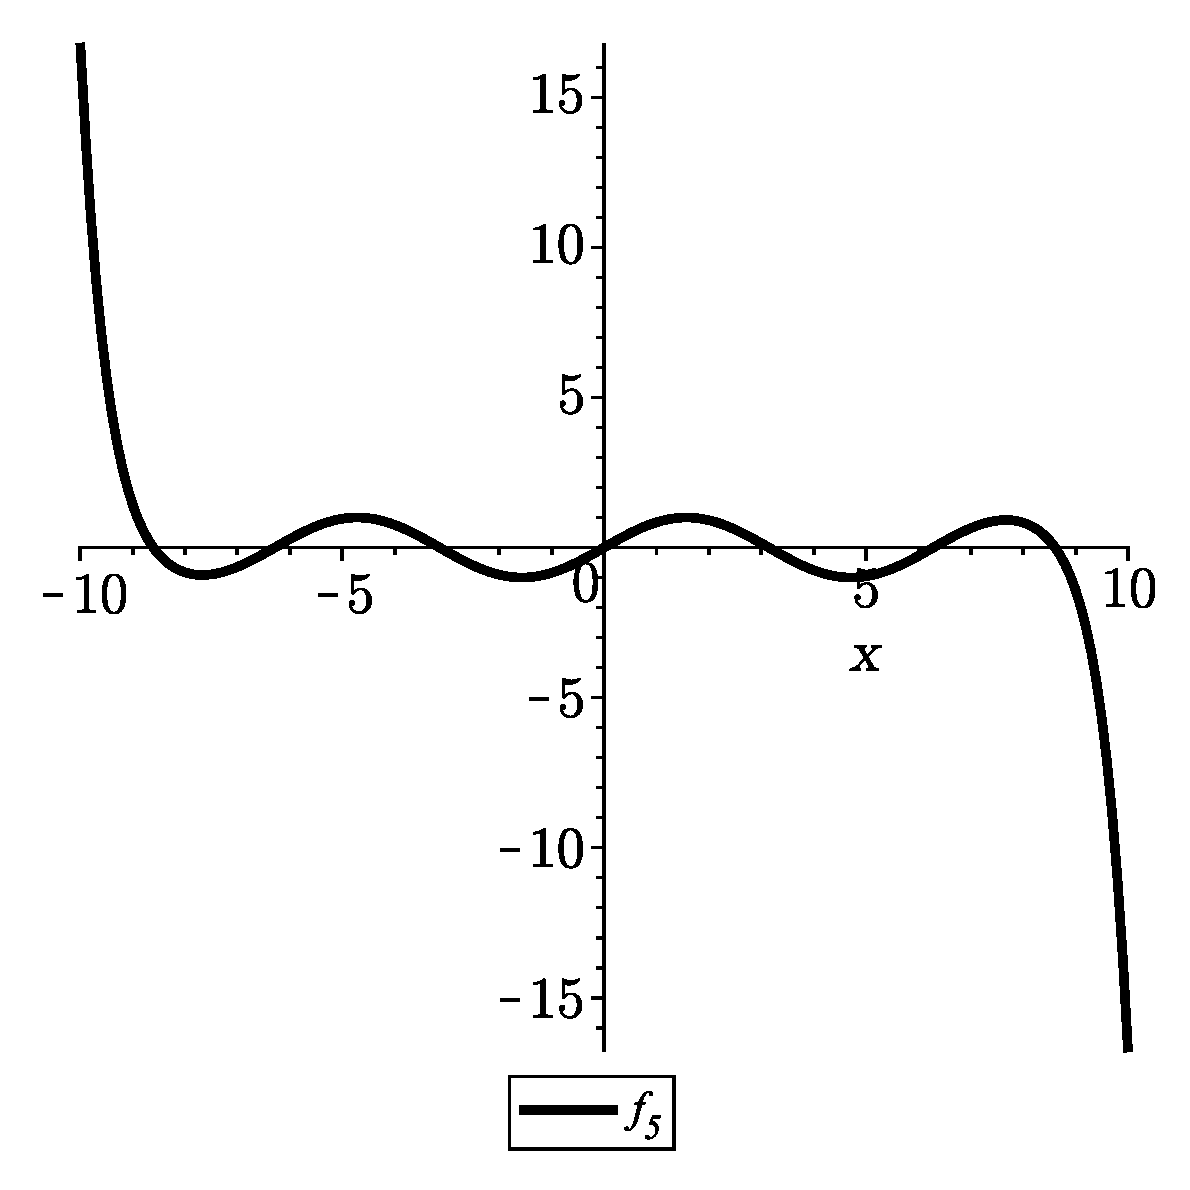
\includegraphics[width=0.7\linewidth]{GraphicalFunctionPlotter/fig/f5Check}
        \caption{Same function as \ref{fig:f5} plotted in Maple.}
        \label{fig:f5Check}
    \end{subfigure}
    \caption{Examples of the PolynomialFunction.}
 \end{figure}


\subsection{\texttt{SumFunction}}
This object takes an array of subclasses of the \texttt{Function} class as parameter. Each subclass in the array then calls its respective \texttt{evaluate} method, and their returned value is added to a running sum. This sum is then returned.

\begin{lstlisting}
double sum = 0;
for(int i = 0; i < f.length; i++){
	sum += f[i].evaluate(x);
}	
return sum;
\end{lstlisting}

If one of these subclasses correspond to a function with large function values, its return values may dominate the sum. Hence the plot may resemble just this particular function. E.g. if we sum a sine wave with values in the interval [$-2.1, \, 2.1$], some other "small-valued" functions, and an exponential function that diverges quickly, the plot may just look like the exponential. This effect is seen on the requested example on figure \ref{fig:f6}.


\begin{figure}[H]
    \begin{subfigure}{0.5\textwidth}
        \centering
        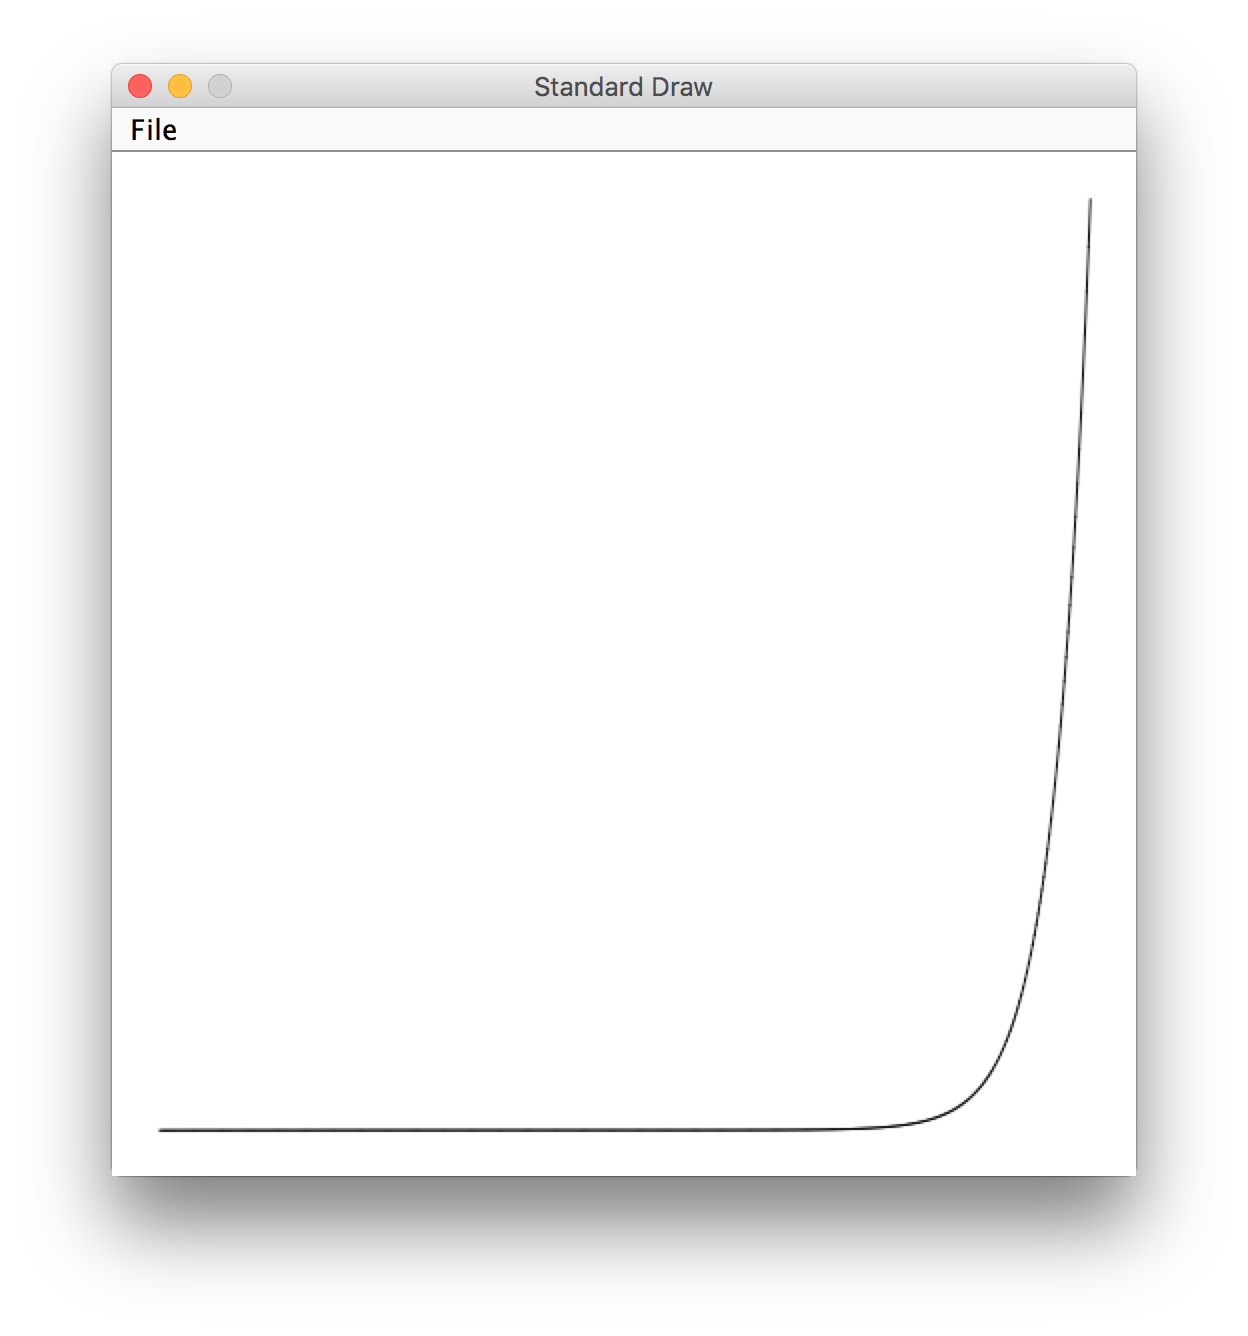
\includegraphics[width=0.7\linewidth]{GraphicalFunctionPlotter/fig/f6.png} 
        \caption{Sum of all previous functions.}
        \label{fig:f6}
    \end{subfigure}
    \begin{subfigure}{0.5\textwidth}
        \centering
        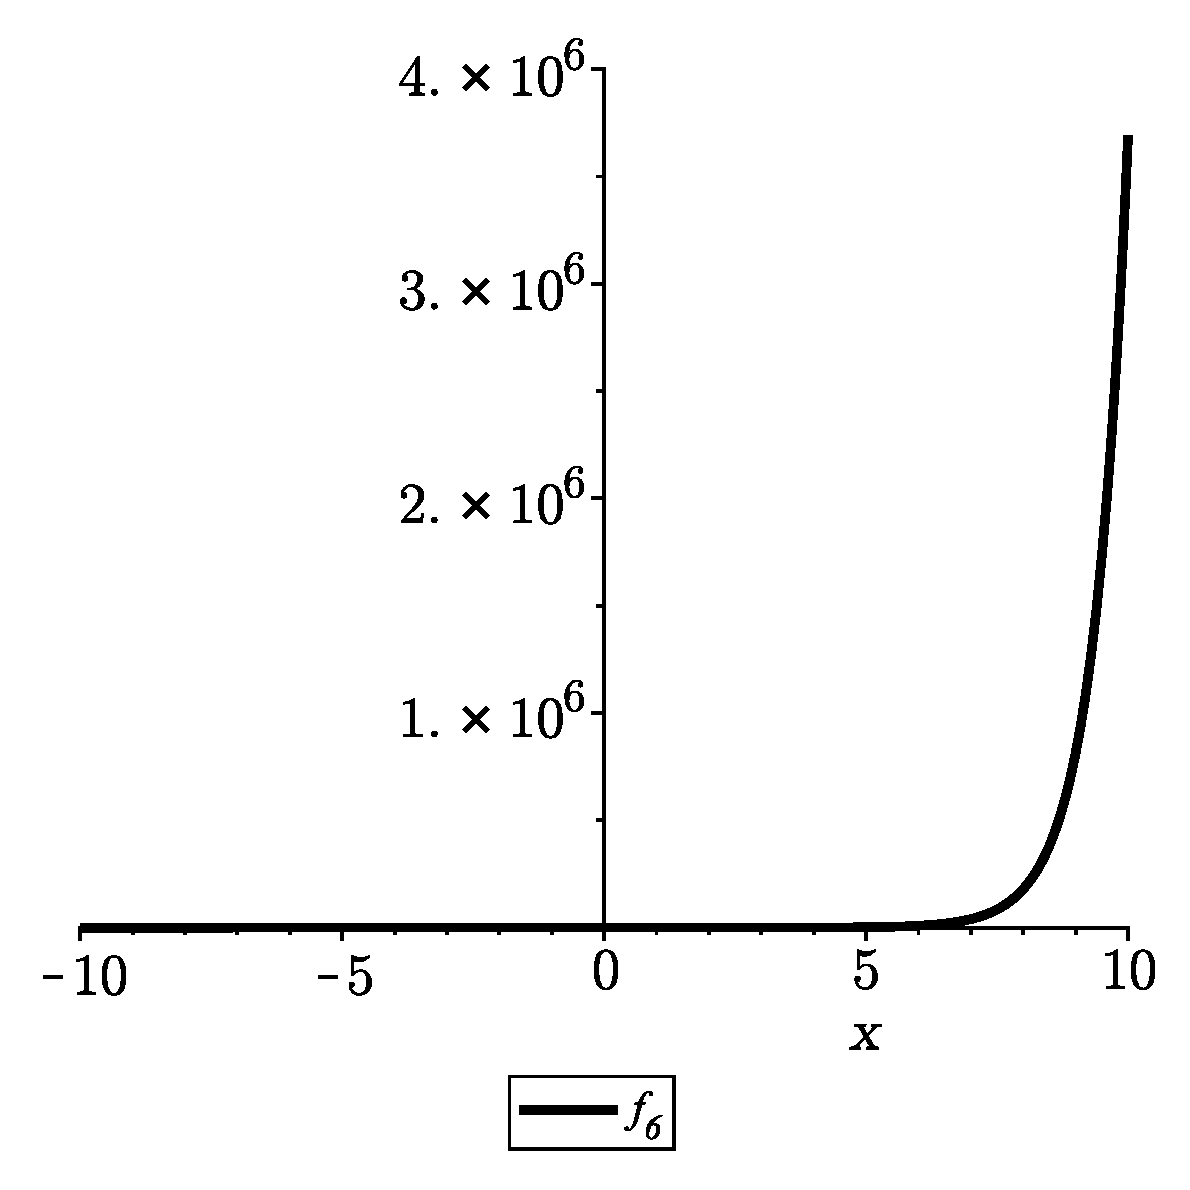
\includegraphics[width=0.7\linewidth]{GraphicalFunctionPlotter/fig/f6Check.eps}
        \caption{Same function plotted in Maple.}
        \label{fig:f6Check}
    \end{subfigure}
    \caption{Examples of the sum functions.}
\end{figure}

\subsection{\texttt{FunctionComposition}}
This object is also given an array of functions as argument. 
When running its \texttt{evaluate} method, it triggers a cascade of method calls using a method called \texttt{value}.

The \texttt{evaluate} method is implemented as follows:

\begin{lstlisting}
public double evaluate(double x) {
	return value(x, 0);
}

private double value(double x, int i){
	if(i >= f.length){
		return x;
	} else {
		return f[i].evaluate(value(x, i+1));
	}
}
\end{lstlisting}

As shown, a recursive method uses \texttt{value}, which creates a stack of functions only collapsing when the base-case is met. In this case, the base-case is, when all functions are put on the stack and \texttt{value} returns x. Each function is then evaluated in the output of the function above it (from the stack perspective), returning the final result through the \texttt{evaluate} method. The requested example is shown in figure \ref{fig:f7}.


\begin{figure}[H]
    \begin{subfigure}{0.5\textwidth}
        \centering
        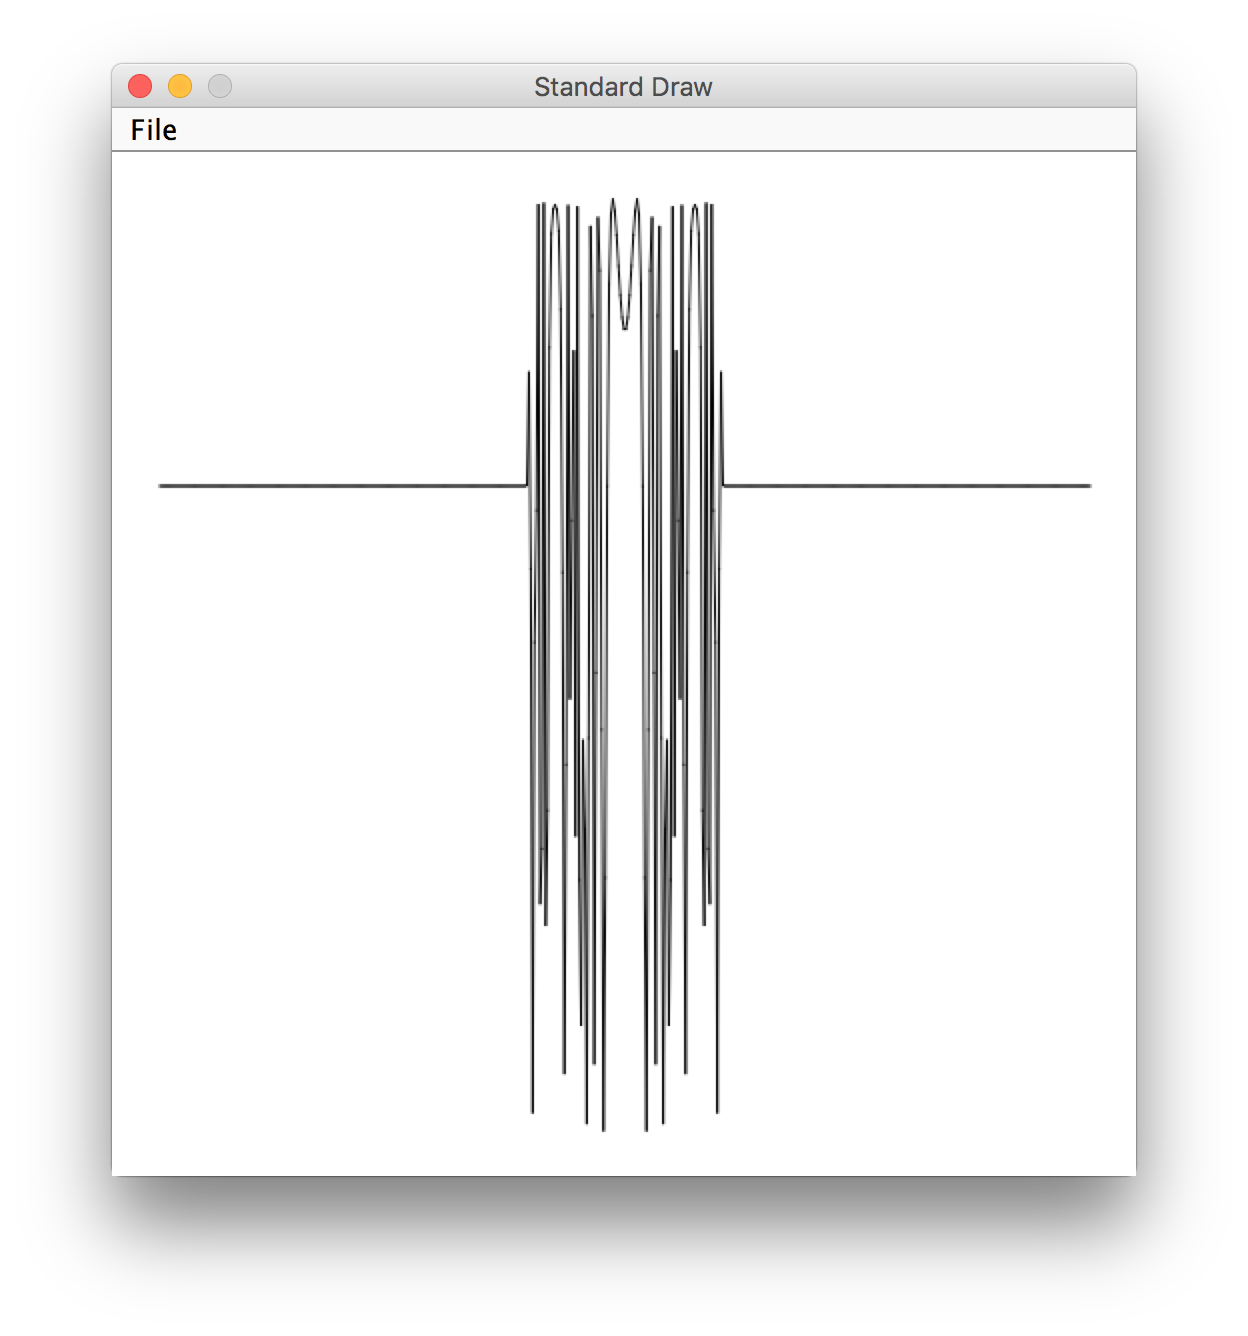
\includegraphics[width=0.7\linewidth]{GraphicalFunctionPlotter/fig/f7.png} 
        \caption{$f_4(f_1(f_3(f_5(f_2(x)))))$.}
        \label{fig:f7}
    \end{subfigure}
    \begin{subfigure}{0.5\textwidth}
        \centering
        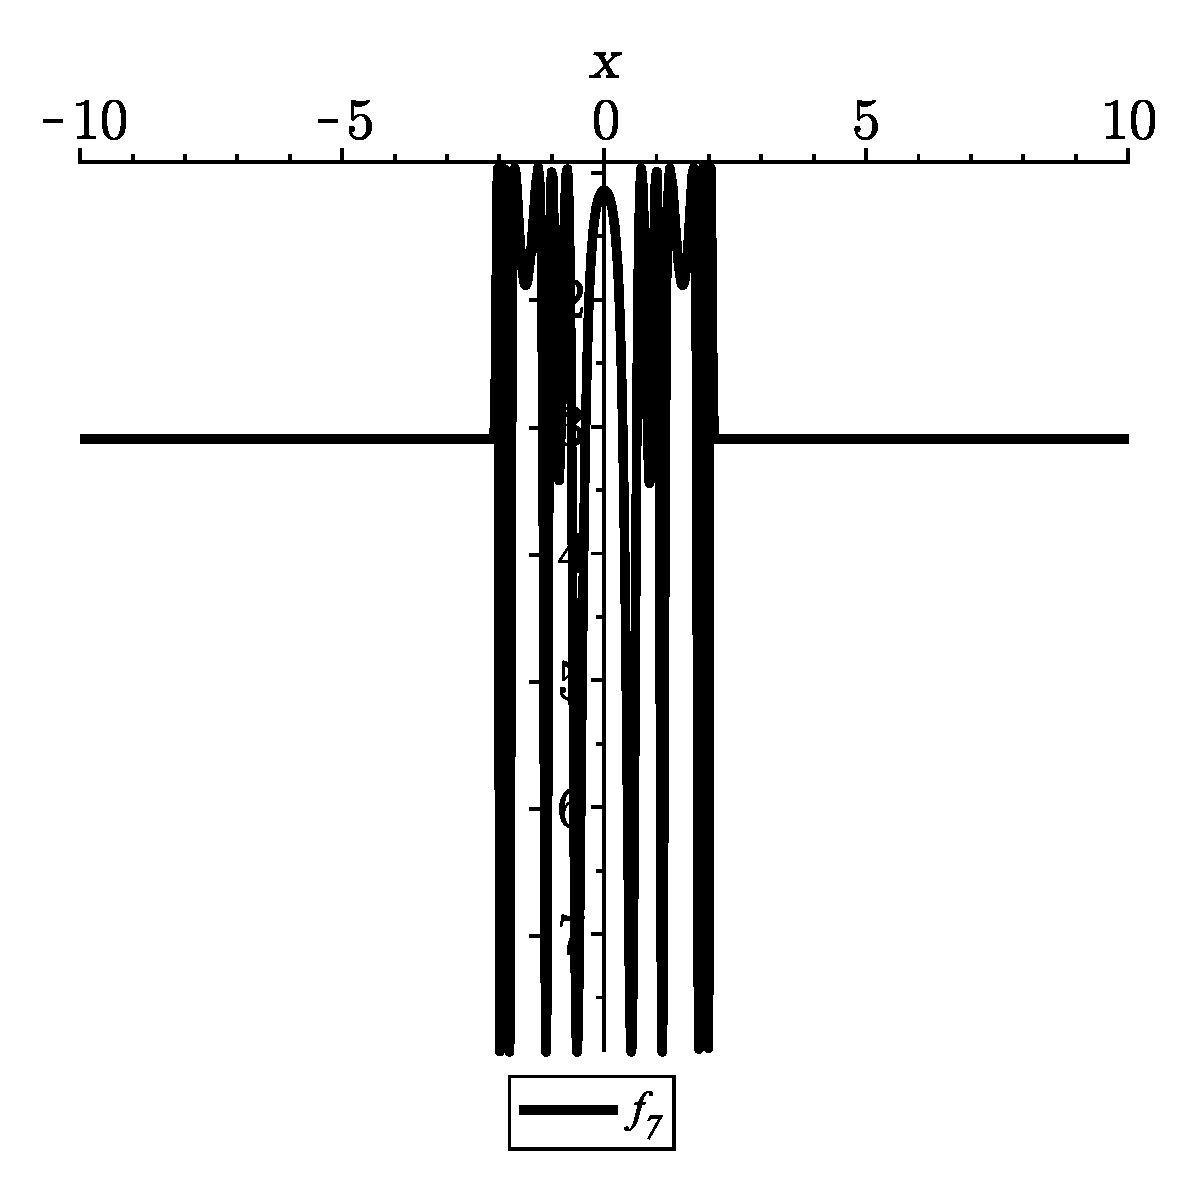
\includegraphics[width=0.7\linewidth]{GraphicalFunctionPlotter/fig/f7Check.eps}
        \caption{Same function plotted in Maple.}
        \label{fig:f7Check}
    \end{subfigure}
    \caption{Example of the composition function.}
\end{figure}

The \texttt{FunctionComposition} class is checked with several combinations of different functions as argument. In most cases, the implemented class and Maple return the same graphs, and hence outputs.\\
\\
However: some combinations of functions do not return the same graphs. We have noticed that these differences occur when power functions and especially exponential functions are compounded. We reckon that the problem is an overflow or precision error when calculating extreme numbers. An example of discrepancy is shown in figure \ref{fig:disc}.

\begin{figure}[H]
    \begin{subfigure}{0.5\textwidth}
        \centering
        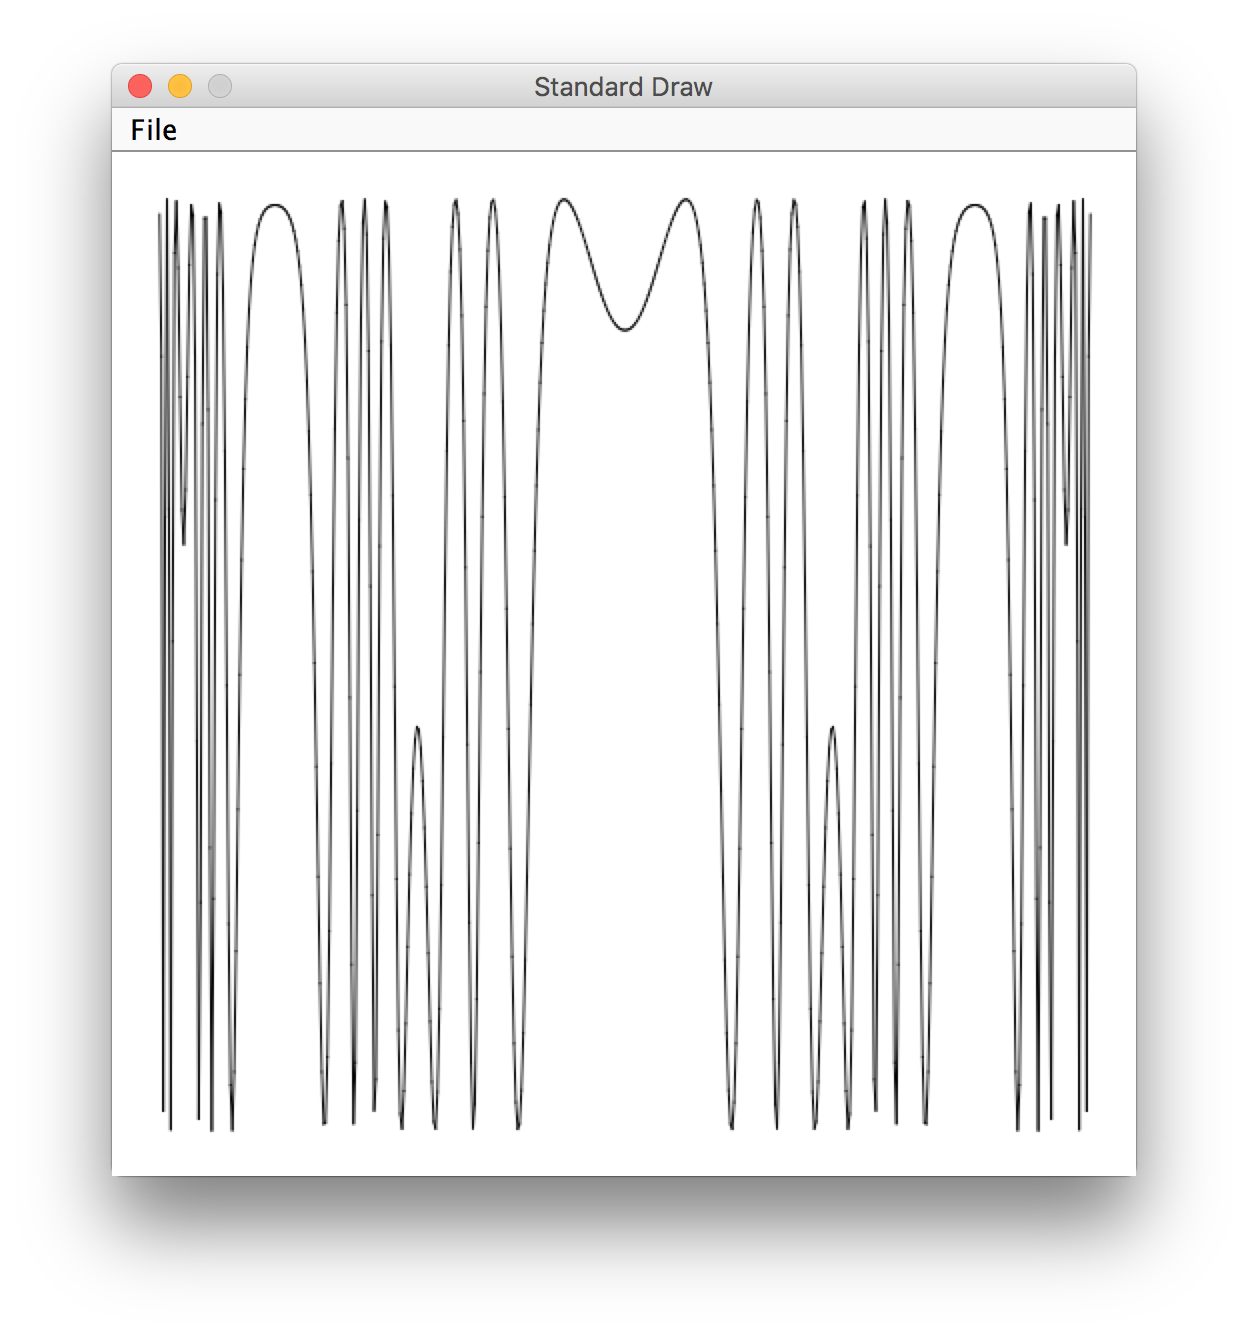
\includegraphics[width=0.7\linewidth]{GraphicalFunctionPlotter/fig/f7Crude.png} 
        \caption{$f_4(f_1(f_3(f_5(f_2(x)))))$. With x from -2 to 2.}
        \label{fig:f7Crude}
    \end{subfigure}
    \begin{subfigure}{0.5\textwidth}
        \centering
        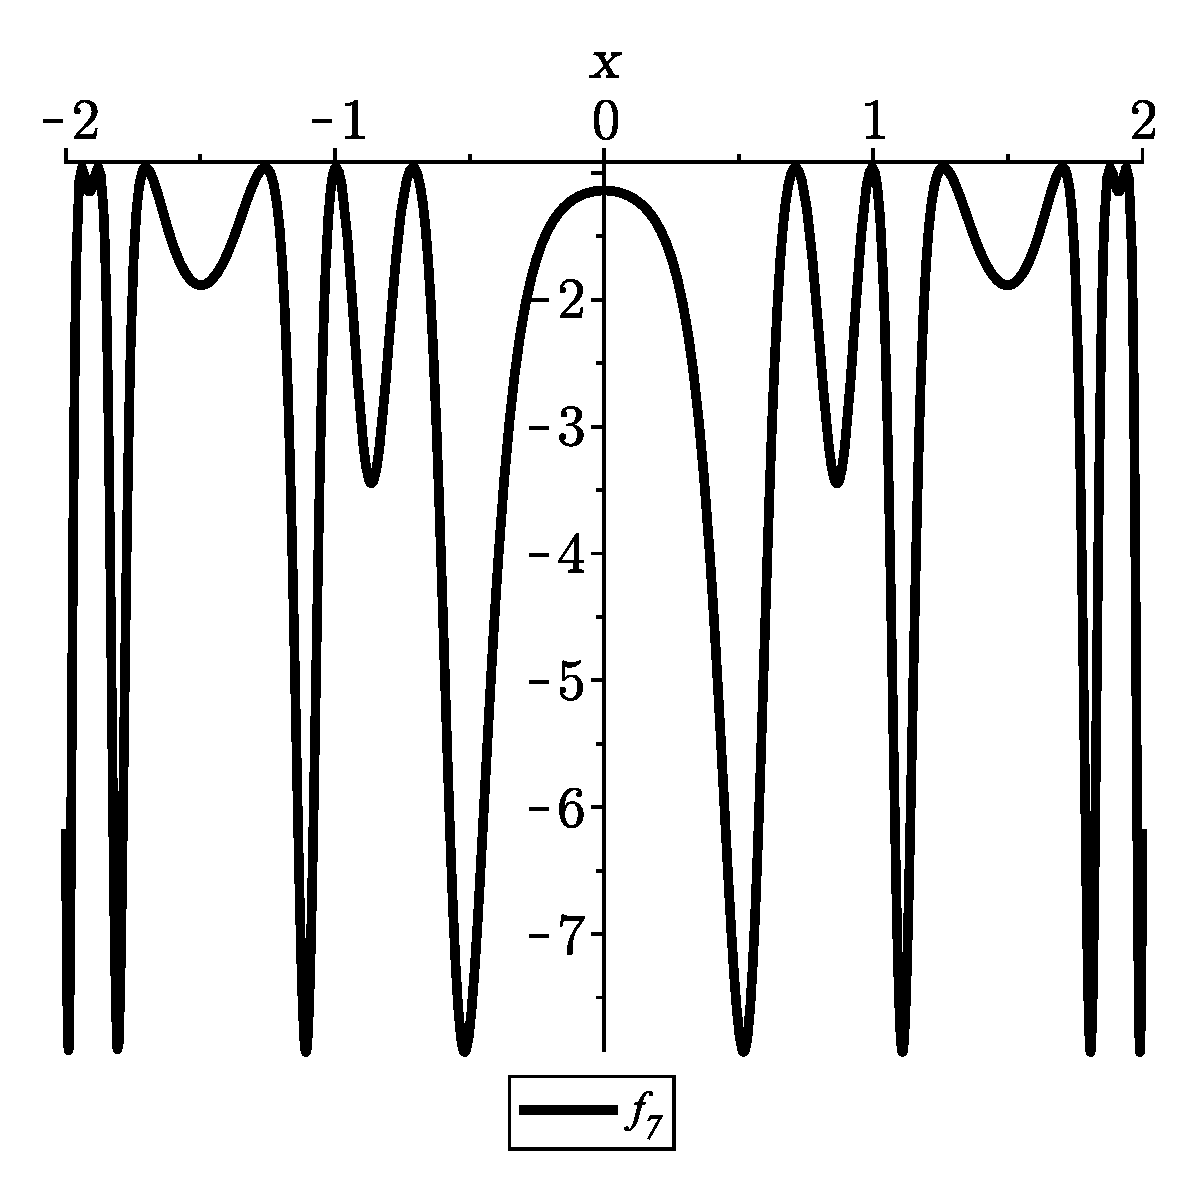
\includegraphics[width=0.7\linewidth]{GraphicalFunctionPlotter/fig/f7CheckCrude.eps}
        \caption{Same function plotted in Maple.}
        \label{fig:f7CheckCrude}
    \end{subfigure}
    \caption{The same function as figure \ref{fig:f7} with a shorter interval.}
    \label{fig:disc}
\end{figure}

\section{Traffic simulation}
We simulated several vehicles which drive on a set track. All vehicles extend an abstract \texttt{Vehicle} super class. The class diagram for the super and subclasses is seen in figure \ref{fig:ClassDiagram}. The subclasses have fields and methods in common, so we implemented the basic fields and methods in the super class to reduce redundancy.

\begin{figure}[H]
    \centering
    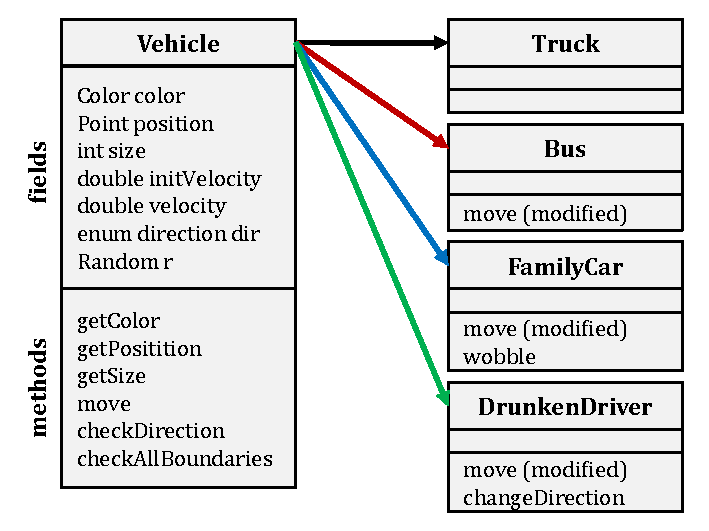
\includegraphics[width=0.7\textwidth]{TrafficSimulation/fig/classDiagram.pdf}
    \caption{Class diagram for \texttt{Vehicle} and its subclasses. \texttt{Truck} is the only vehicle which uses the default \texttt{move} method. All subclasses contain the same fields.}
    \label{fig:ClassDiagram}
\end{figure}

As seen in figure \ref{fig:ClassDiagram} they all extend a template for the \texttt{move} method. This method by default defines a perfectly symmetrical movement counterclockwise around the track. Since all vehicles except \texttt{DrunkenDriver} mainly follows this pattern, it is placed in the super class. The deviations from the default moving pattern is implemented in each subclass. \\
\\
For example: The bus moves like the truck, except in the special case when the bus is in the bottom lane, moving to the right. Hence we implemented the \texttt{move} method in Bus by first calling the \texttt{move} method from \texttt{Vehicle}, and then the special case:

\begin{lstlisting}
public void move() {
// the super class has the default move method used by Truck
super.move();
// if bus is in bottom lane (moving right), move at faster velocity
switch (dir) {
	case RIGHT:
		velocity = 1.6 * initVelocity;
		break;
	default:
		velocity = initVelocity;
...
\end{lstlisting}

\subsection{Collision avoidance}
The \texttt{Vehicle} class also contains some methods to avoid going outside the legal track, as seen on figure \ref{fig:ClassDiagram}. \texttt{checkDirection} is used to check whether a move in the current direction is possible without going outside the track. \\
\texttt{checkAllBoundaries} performs additional checks; it includes checks to keep the vehicle from colliding with the inner ring.\\
\\
All vehicles on the track are shown in figure \ref{fig:traffic1}. As seen on this figure, there is no collision detection between the individual vehicles; they may pass freely through each other. 

\begin{figure}[H]
    \centering
    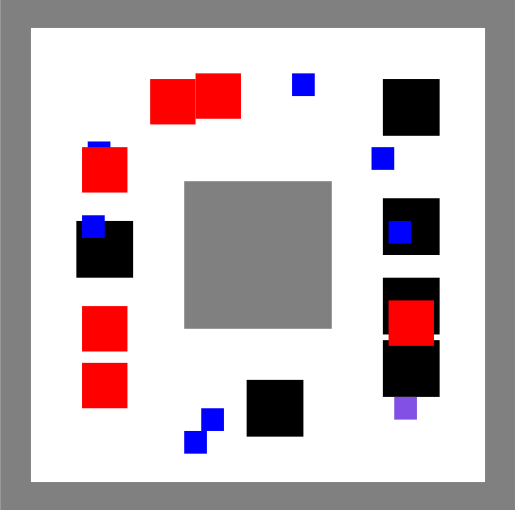
\includegraphics[width=0.7\textwidth]{TrafficSimulation/fig/traffic3}
    \caption{A test run of our traffic simulation.}
    \label{fig:traffic1}
\end{figure}

The subclasses are described in more detail below:

\subsection{\texttt{Truck}}
The \texttt{Truck} subclass is the simplest of all the vehicles. It drives around the track with constant velocity, is the slowest of all vehicles, and the larges. It follows the default move pattern exactly, changing direction when it crosses the center of each corner in a counterclockwise motion.\\

\textbf{Specifications:}
\begin{itemize}
    \item Velocity: 1
    \item Color: Black
    \item Size: 5
\end{itemize}

The \texttt{Truck} should always be the slowest vehicle on the track, so we sets its velocity 
\subsection{\texttt{Bus}}
The \texttt{Bus} and Truck are much alike. The main difference is that the \texttt{Bus}' velocity is not constant on all edges. The \texttt{Bus} speeds up on the bottom edge. 

The \texttt{Bus} is slightly smaller than the \texttt{Truck}, and slightly faster.\\

Specifications:
\begin{itemize}
    \item Velocity: 2 (3 on bottom edge)
    \item Color: \textcolor{red}{Red}
    \item Size: 4
\end{itemize}

\subsection{\texttt{FamilyCar}}
The \texttt{FamilyCar} is more customized than the previous subclasses. It implements the move method from \texttt{Vehicle} but also implements a \texttt{wobble} method which ensures that there is random chance of a deviation from the default moving pattern.\\
\\
The \texttt{FamilyCar} also has a random chance of changing its velocity on each move.
The new velocity is based on the initial velocity (which is preset) and a randomly generated integer.\\

\textbf{Specifications:}
\begin{itemize}
    \item Velocity: 2-4
    \item Color: \textcolor{blue}{Blue}
    \item Size: 2
\end{itemize}

\subsection{\texttt{DrunkenDriver}}
This vehicle is completely chaotic. \texttt{DrunkenDriver} does not use the default movement pattern, so it has a unique \texttt{move} method. As a result, other boundary checking methods were needed.\\
\\
In the beginning of each \texttt{move} method call, the drunk attempts to move forward in its current direction. The new position is checked with one of the boundary checking methods from the \texttt{Vehicle} class. If the drunk would end up inside a wall, it moves backwards instead.\\
\\
\textbf{How the boundary check is performed:}\\
%If this method returns true, the new position is not in danger of colliding with the side or inner walls. 
The method \texttt{checkAllBoundaries} checks whether the position plus vehicle size plus a full step would intersect an illegal area, and returns true of the move is legal. \\

\textbf{Changing directions:}\\
If the \texttt{checkAllBoundaries} returns false, the \texttt{DrunkenDriver} is translated 2 $\cdot$ \texttt{velocity} backwards, and the drunk has a 100 \% chance of choosing a random direction for its next move.\\
\\
After each \texttt{move} method call, no matter if the drunk was close to a wall or not, the \texttt{DrunkenDriver} has a 10 \% chance of choosing a random direction.\\
\\
\textbf{Specifications:}
\begin{itemize}
    \item Velocity: 2-4
    \item Color: Varying color
    \item Size: 2
\end{itemize}







\end{document}

